\section{Understanding $PPF_{fuel}$}

Equation \ref{eq:reaction-rate-fission} shows the relationship between fission reaction rate, 
flux, and material properties. 
\begin{align}
\label{eq:reaction-rate-fission}
    RR_f &= \Phi \times \sigma_f \times N \\
\intertext{where}
    RR_f &= \mbox{fission reaction rate } [reactions \cdot cm^{-3} \cdot s^{-1}]\nonumber \\
    \Phi &= \mbox{neutron flux } [neutrons \cdot cm^{-2} \cdot s^{-1}] \nonumber \\
    \sigma_f &= \mbox{microscopic cross section } [cm^2] \nonumber \\
    N &= \mbox{atomic number density } [atoms \cdot cm^{-3}] \nonumber 
\end{align}

Since microscopic cross section is constant for the same fuel material, we can rearrange 
Equation \ref{eq:reaction-rate-fission} into Equation \ref{eq:reaction-rate-fission-prop}: 
\begin{align}
    \label{eq:reaction-rate-fission-prop}
    \Phi \propto \frac{RR_f}{N}
    \intertext{where}
    \Phi &= \mbox{neutron flux } [neutrons \cdot cm^{-2} \cdot s^{-1}] \nonumber \\
    RR_f &= \mbox{fission reaction rate } [reactions \cdot cm^{-3} \cdot s^{-1}]\nonumber \\
    N &= \mbox{atomic number density } [atoms \cdot cm^{-3}] \nonumber
\end{align}
In Section \ref{sec:ahtr_slab_output}, I defined $PPF_{fuel}$ as: 
\begin{align}
    PPF_{fuel} &= max(\frac{fqr_j}{PF_j}) \div ave(\frac{fqr_j}{PF_j})
\intertext{where}
j &= \mbox{discretized fuel area j} \nonumber \\
PPF_{fuel} &= \mbox{fuel-normalized power peaking factor} \nonumber \\
fqr_j &= \mbox{fission-q-recoverable at position j} \nonumber \\
PF_j &= \mbox{fuel packing fraction at position j} \nonumber
\end{align}
The fission reaction rate ($RR_f$) is proportional to fission energy production rate ($fqr$). 
The atomic number density (N) is proportional to the fuel packing fraction ($PF$). 
Thus, we can further rearrange Equation \ref{eq:reaction-rate-fission-prop} into 
Equation \ref{eq:flux-prop-fqr}:
\begin{align}
    \label{eq:flux-prop-fqr}
    \Phi_j \propto \frac{fqr_j}{PF_j}
    \intertext{where}
    \Phi &= \mbox{neutron flux at position j} [neutrons \cdot cm^{-2} \cdot s^{-1}] \nonumber \\
    fqr_j &= \mbox{fission-q-recoverable at position j} \nonumber \\
    PF_j &= \mbox{fuel packing fraction at position j} \nonumber
\end{align}

An overall flatter plank thermal flux from Group 4 (see Table \ref{tab:fission-flux}) will 
result in a lower fuel-normalized power peaking factor. 
Table \ref{tab:fission-flux} shows the percentage contributions of fission reactions from 
each energy group. 
\begin{table}[H]
    \centering
    \onehalfspacing
    \caption{Percentage of fission reactions from each energy group for \gls{AHTR} plank model.}
	\label{tab:fission-flux}
    \footnotesize
    \begin{tabular}{llp{4cm}}
    \hline 
    \textbf{Energy Group} & \textbf{sBound} & \textbf{Percentage of Total Fission Reactions [\%]} \\
    \hline
    1 & $9.1188\times 10^{-3} < E < 2.0000\times 10^1$ & 0.85 \\ 
    2 & $2.9023\times 10^{-5} < E < 9.1188\times 10^{-3}$ & 4.85 \\
    3 & $1.8554\times 10^{-6} < E < 2.9023\times 10^{-5}$ & 4.14 \\
    4 & $1.0000\times 10^{-12} < E < 1.8554\times 10^{-6}$ & 90.14 \\
    \hline
    \end{tabular}
\end{table}
Most fission reactions are occurring in Energy Group 4. 

\subsection{Simulation p-1c: Variation of $\rho_{TRISO}(\vec{r})$ to minimize $PPF_{fuel}$}
Table \ref{tab:simulationp1c} shows simulation p-1c's optimization problem parameters. 
\begin{table}[H]
    \centering
    \onehalfspacing
    \caption{Simulation p-1c Optimization Problem Parameters}
	\label{tab:simulationp1c}
    \footnotesize
    \begin{tabular}{l|p{3cm}}
    \hline 
    \multicolumn{2}{c}{\textbf{Single Objective: Simulation p-1c}} \\
    \hline 
    \textbf{Objectives} & Minimize $PPF_{fuel}$ \\
    \hline 
    \textbf{Input parameter variations} & $0<a<2$ \\
    & $0<b<\frac{\pi}{2}$ \\
    & $0<c<2\pi$ \\
    \hline
    \textbf{Constraints} & $k_{eff} \geq 1.0$\\ 
    & $PF_{total}$ = 0.0979\\
    \hline 
    \textbf{Genetic algorithm parameters} & Population size: 60 \\
    & Generations: 10 \\
    \hline
    \end{tabular}
\end{table}

Figure \ref{fig:slab-obj-1-ppf-evol} shows the plank's $PPF_{fuel}$ evolution, 
Figure \ref{fig:slab-obj-1-ppf-final} shows the five \gls{TRISO} 
packing fraction distributions ($\rho_{TRISO}(\vec{r})$) in the final generation 
with the most-minimized $PPF_{fuel}$, and Figure 
\ref{fig:slab-obj-1-ppf-most-minimized} illustrates the \gls{AHTR} plank model with 
most-minimized $PPF_{fuel}$. 
\begin{figure}[H]
    \centering
    \begin{subfigure}{0.9\textwidth}
        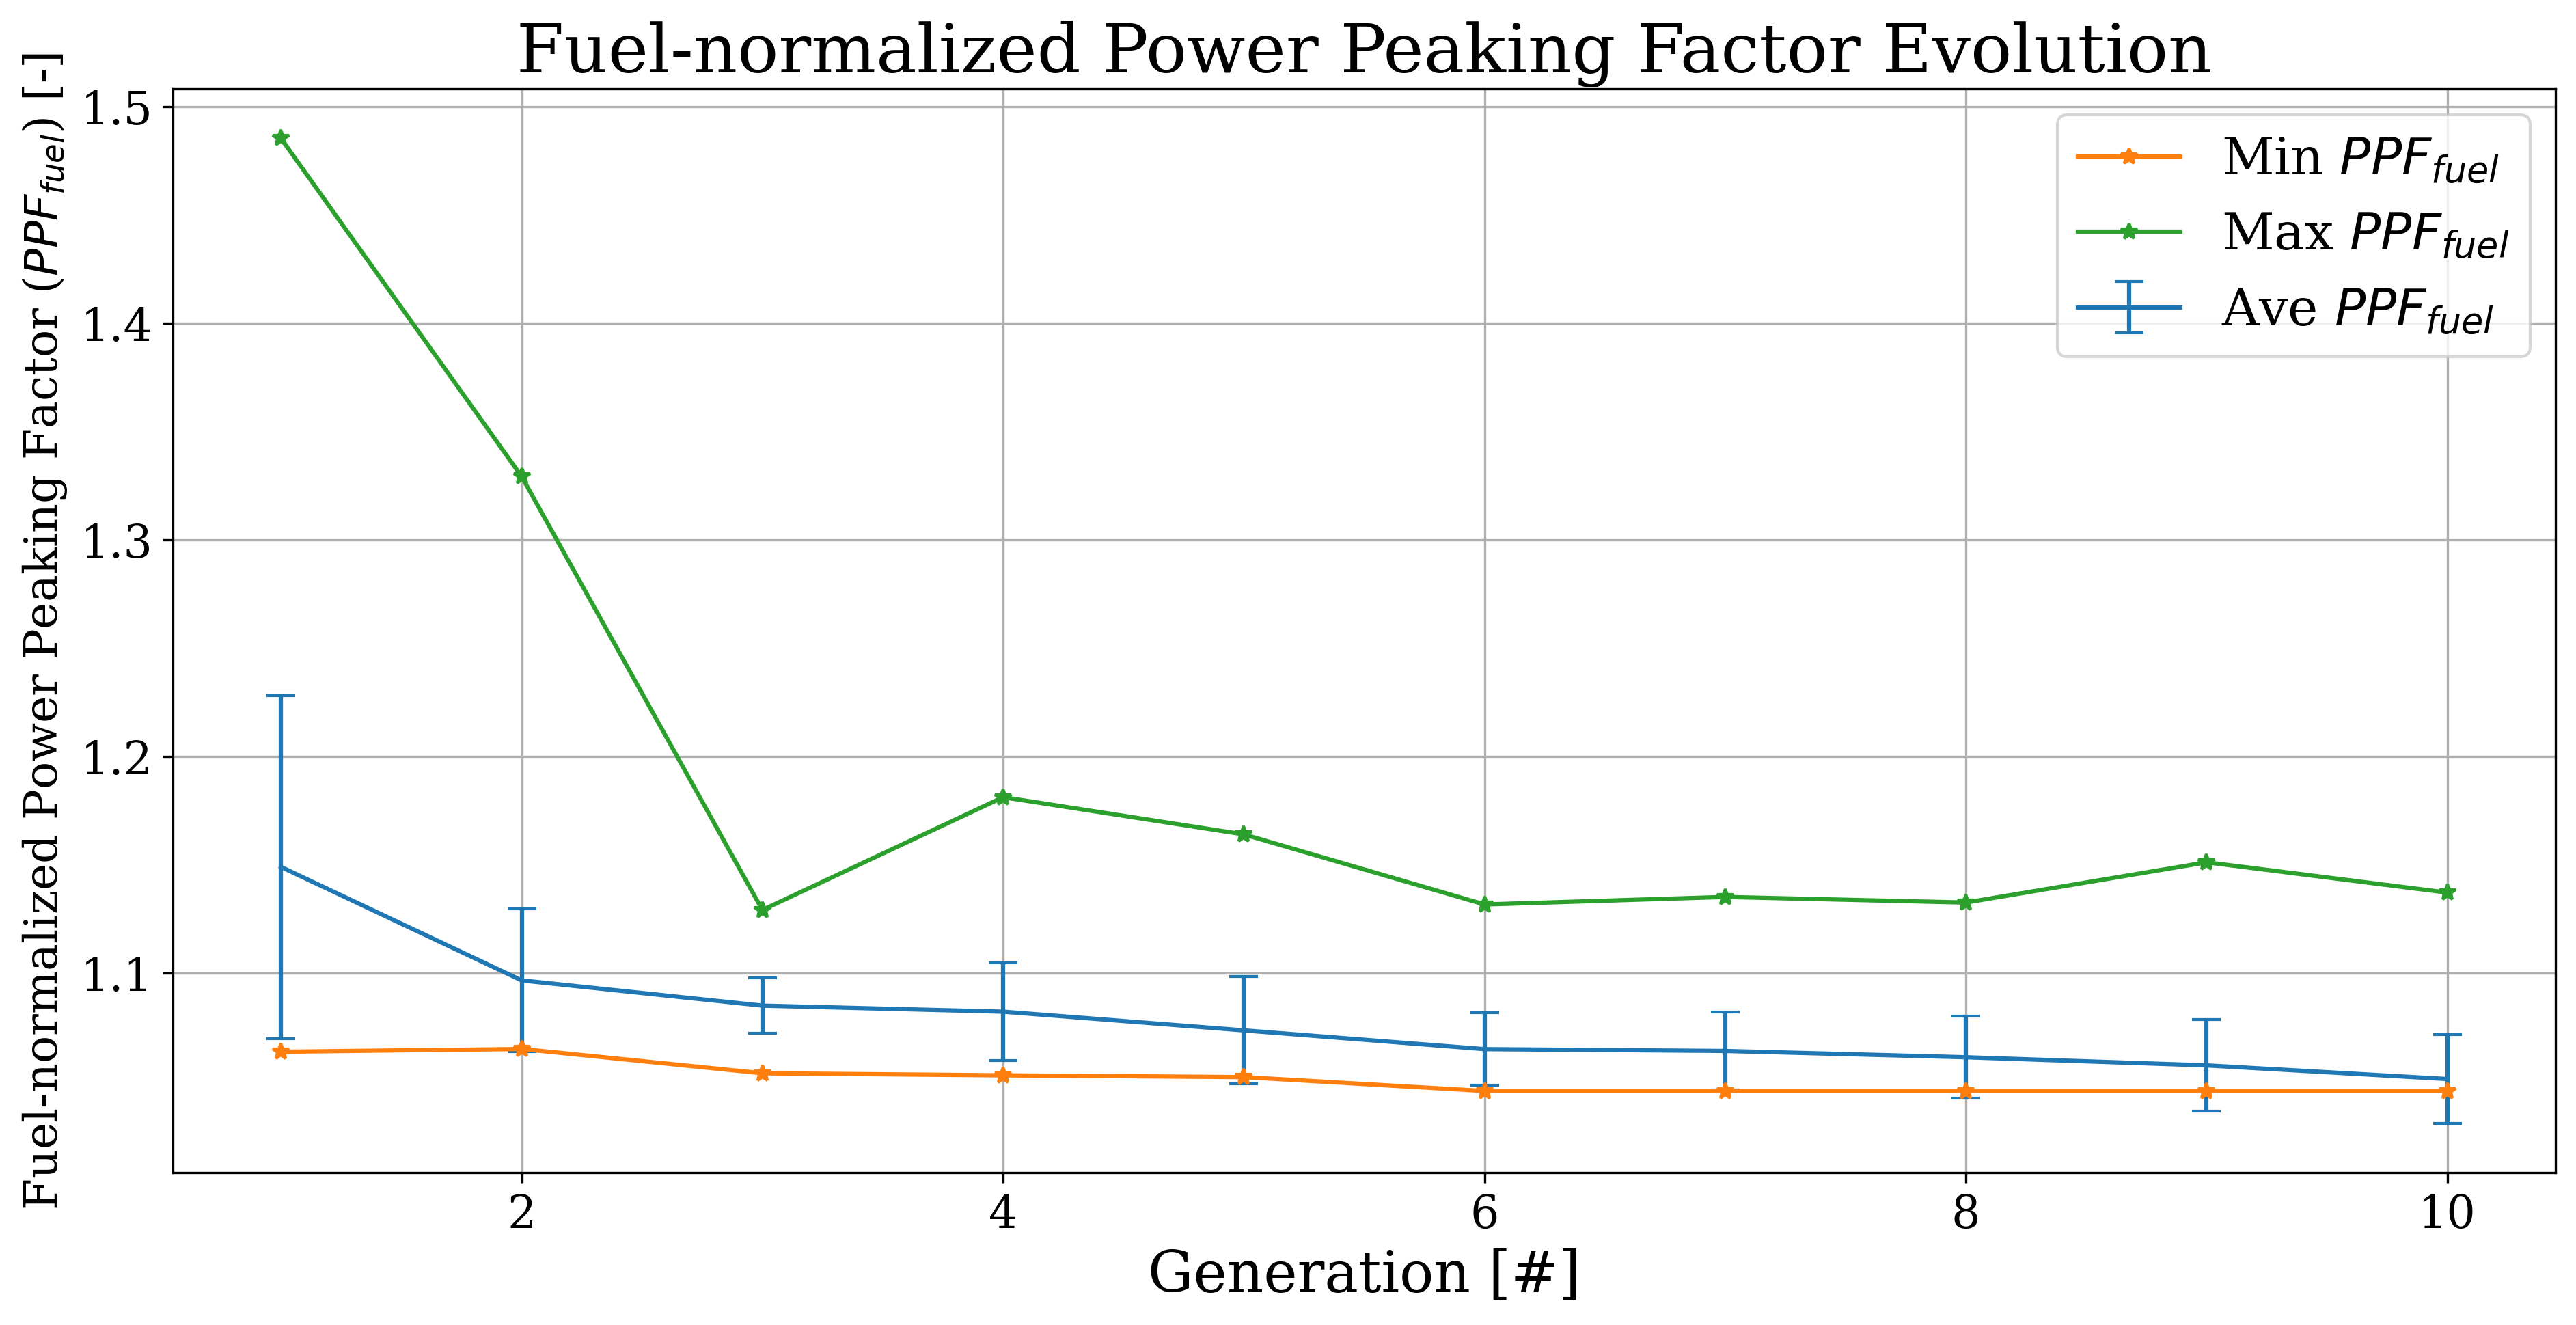
\includegraphics[width=\linewidth]{slab-obj-1-ppf-evol.png}
        \caption{Minimum, average, and maximum evolution of $PPF_{fuel}$ in the 
        AHTR plank.}
        \label{fig:slab-obj-1-ppf-evol} 
    \end{subfigure}
    \begin{subfigure}{0.9\textwidth}
        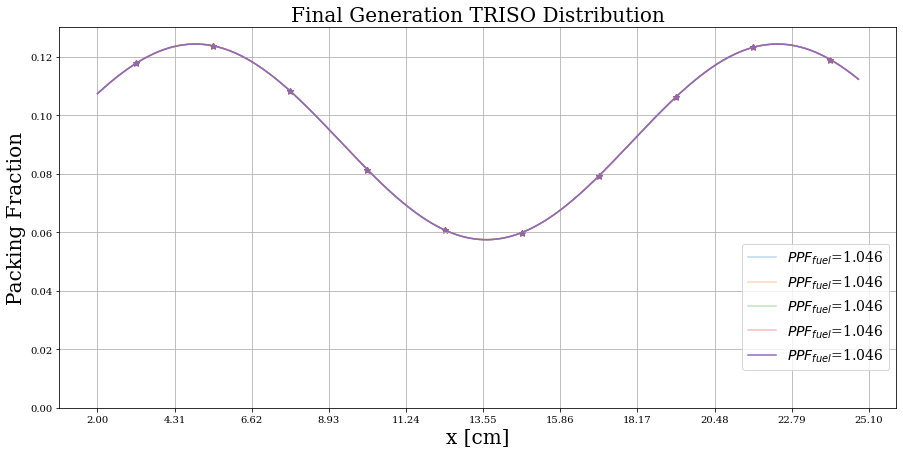
\includegraphics[width=\linewidth]{slab-obj-1-ppf-final.png}
        \caption{TRISO distribution for the 5 reactor models with the 
        lowest $PPF_{fuel}$ in AHTR plank at the final generation.}
        \label{fig:slab-obj-1-ppf-final} 
    \end{subfigure}
    \begin{subfigure}{0.9\textwidth}
        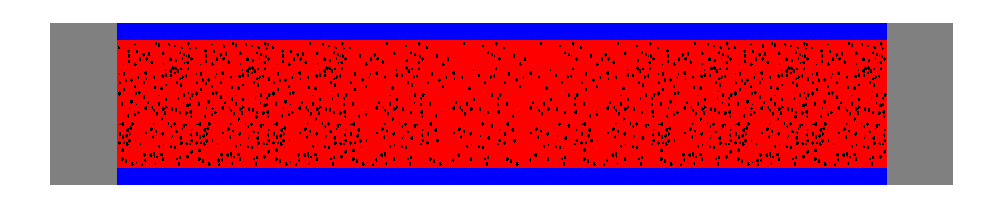
\includegraphics[width=\linewidth]{slab-obj-1-ppf-most-minimized.png}
        \caption{\gls{AHTR} plank model with most-minimized $PPF_{fuel}$
        (corresponds to the purple bolded distribution in the above plot).}
        \label{fig:slab-obj-1-ppf-most-minimized} 
    \end{subfigure}
    \caption{Simulation p-1c -- ROLLO single-objective optimization to minimize 
    AHTR plank's fuel-normalized power peaking factor ($PPF_{fuel}$). 
    Input parameters varied: TRISO distribution ($\rho_{TRISO}(\vec{r})$).
    $PF_{total}$ = 0.0979.}
    \label{fig:slab-obj-1-ppf}
\end{figure}

In Figure \ref{fig:slab-obj-1-ppf-final}, the TRISO distribution that best minimizes 
$PPF_{fuel}$ peaks near the edges of the fuel region of the plank, and has a minimum 
point in center of the plank.
This distribution is attributed to \gls{ROLLO} trying to flatten thermal flux in 
the plank to minimize fuel-normalized power peaking factor. 

Figure \ref{fig:flux-comparison-0.0979-plank} compares the flux distributions from the 
Figure \ref{fig:slab-obj-1-ppf-final}'s TRISO distribution and a constant 
$PF_{total}$ = 0.0979 TRISO distribution. 
The $PPF_{fuel}$ value for constant $PF_{total}$ = 0.0979 TRISO distribution is 1.089. 
\begin{figure}[H]
    \centering
    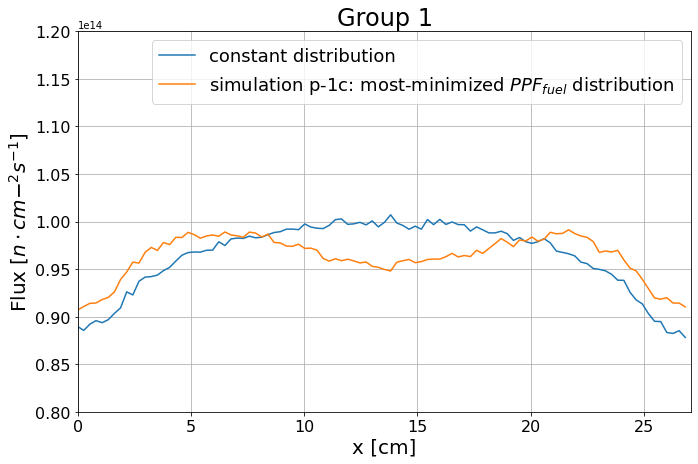
\includegraphics[width=0.48\linewidth]{flux-comparison-0.0979-plank_grp1.png} 
    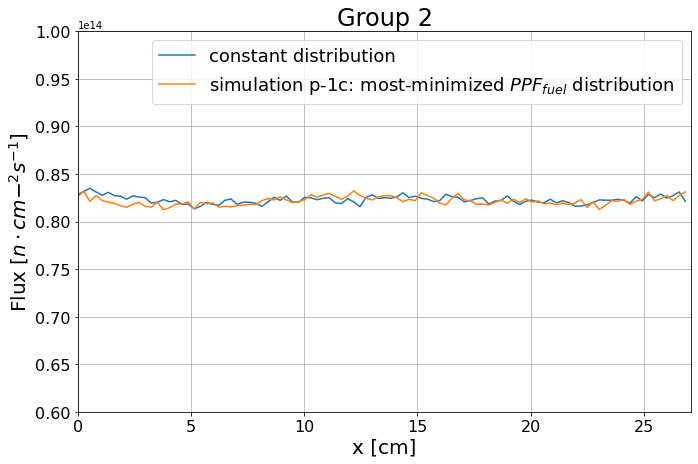
\includegraphics[width=0.48\linewidth]{flux-comparison-0.0979-plank_grp2.png} 
    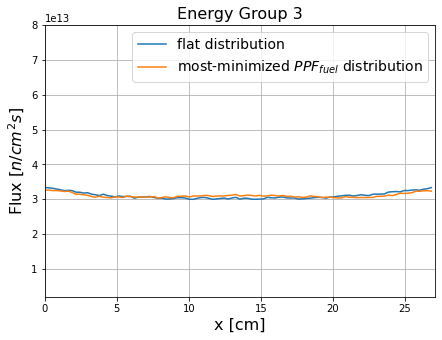
\includegraphics[width=0.48\linewidth]{flux-comparison-0.0979-plank_grp3.png} 
    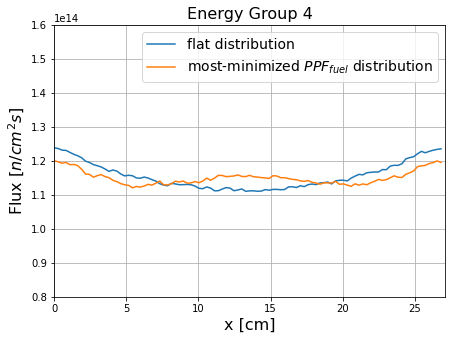
\includegraphics[width=0.48\linewidth]{flux-comparison-0.0979-plank_grp4.png} 
    \caption{Flux comparison between Figure \ref{fig:slab-obj-1-ppf-final}'s TRISO 
    distribution that most-minimized $PPF_{fuel}$ and a constant $PF_{total}$ = 0.0979 
    TRISO distribution. 
    \acrfull{AHTR} plank's centerline neutron flux distribution in 4 groups at 948K. 
    Centerline is the white line in Figure \ref{fig:ahtr-plank-verification}.
    Energy Group 1: E $> 9.1188 \times 10^{-3}$ MeV, 
    Energy Group 2: $2.9023 \times 10^{-5} < E < 9.1188 \times 10^{-3}$ MeV,
    Energy Group 3:  $1.8556 \times 10^{-5} < E < 2.9023 \times 10^{-5}$ MeV,
    Energy Group 4:  $1.0 \times 10^{-12} < E < 1.8554 \times 10^{-6}$ MeV.}
    \label{fig:flux-comparison-0.0979-plank}
\end{figure}
In Energy group 4, the most-minimized $PPF_{fuel}$ flux distribution is 0.96x flatter 
than the constant $PF_{total}$ = 0.0979 flux distribution, resulting in a lower 
$PPF_{fuel}$. 
The dip in the constant $PF_{total}$ = 0.0979 thermal flux distribution is due to 
self-shielding effects. 

\subsection{p-2b: Minimize $PF_{total}$ and $PPF_{fuel}$}
\label{sec:p-2b}
This section reports results from the two-objective optimization simulation p-2b, the 
objectives minimized are total fuel packing fraction ($PF_{total}$) and fuel-normalized 
power peaking factor ($PPF_{fuel}$).  
Table \ref{tab:simulationp2b} shows simulation p-2b's optimization problem parameters. 
\begin{table}[H]
    \centering
    \onehalfspacing
    \caption{Simulation p-2b Optimization Problem Parameters}
	\label{tab:simulationp2b}
    \footnotesize
    \begin{tabular}{l|p{3cm}}
    \hline 
    \multicolumn{2}{c}{\textbf{Two Objectives: Simulation p-2b}} \\
    \hline 
    \textbf{Objectives} & Minimize $PF_{total}$ \\
    & Minimize $PPF_{fuel}$ \\
    \hline 
    \textbf{Input parameter variations} & $0.02<PF_{total}<0.04$ \\
    & $0<a<2$ \\
    & $0<b<\frac{\pi}{2}$ \\
    & $0<c<2\pi$ \\
    \hline
    \textbf{Constraints} & $k_{eff} \geq 1.35$\\ 
    \hline 
    \textbf{Genetic algorithm parameters} & Population size: 128 \\
    & Generations: 3 \\
    \hline
    \end{tabular}
\end{table}

Figure \ref{fig:slab-obj-2-pfppf-pareto} shows a plot of the final generation's reactor 
models' $PF_{total}$ against $PPF_{fuel}$, crosses mark the reactor models that fall on 
the Pareto front.
Figure \ref{fig:slab-obj-2-pfppf-pareto-distr} shows the four TRISO packing fraction 
distributions in the final generation that fall on the Pareto front. 
Figures \ref{fig:slab-obj-2-pfppf-min-pf} and \ref{fig:slab-obj-2-pfppf-min-ppf} 
illustrate the \gls{AHTR} plank models with most-minimized $PF_{total}$ and 
$PPF_{fuel}$, respectively. 
\begin{figure}[H]
    \centering
    \begin{subfigure}{\textwidth}
        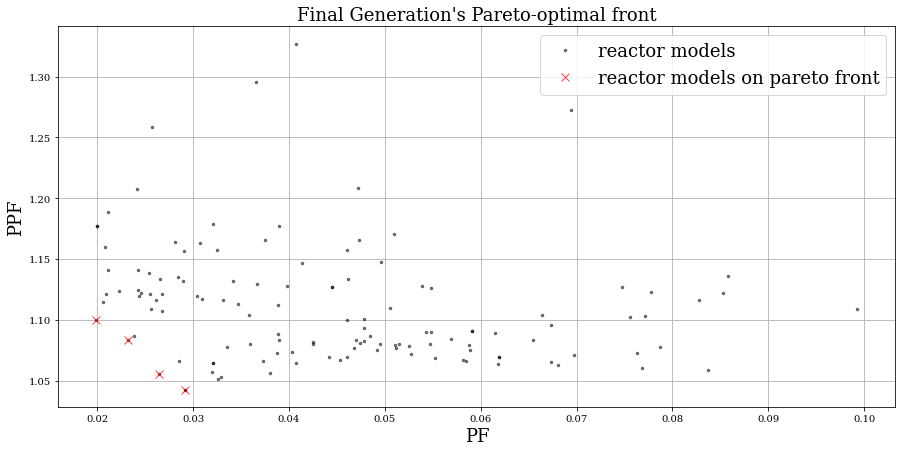
\includegraphics[width=\linewidth]{slab-obj-2-pfppf-pareto.png}
        \caption{Plot of final generation's reactor models' $PF_{total}$ against 
        $PPF_{fuel}$. 
        Crosses indicate the reactor models on the Pareto front. Cross colors correspond  
        to TRISO distributions in the plot below.}
        \label{fig:slab-obj-2-pfppf-pareto} 
    \end{subfigure}
    \begin{subfigure}{\textwidth}
        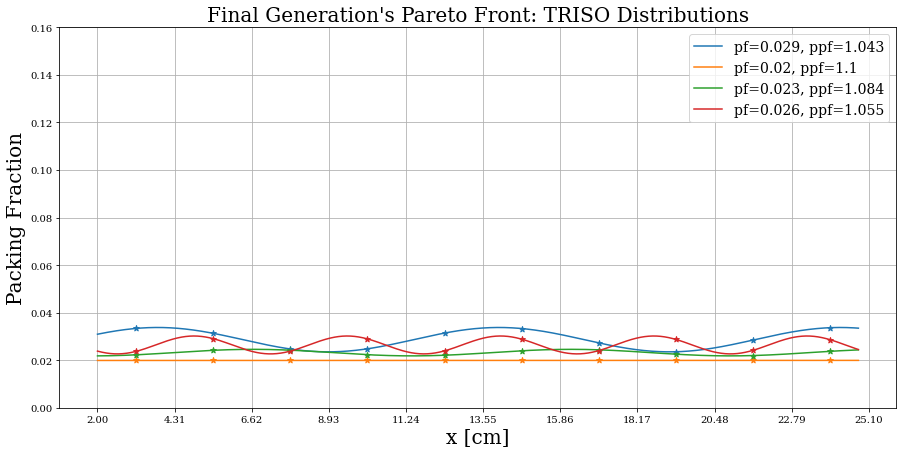
\includegraphics[width=\linewidth]{slab-obj-2-pfppf-pareto-distr.png}
        \caption{TRISO distribution for the 4 reactor models on the Pareto front.}
        \label{fig:slab-obj-2-pfppf-pareto-distr} 
    \end{subfigure}
    \caption{Simulation p-2b -- ROLLO two-objective optimization to minimize total fuel 
    packing fraction ($PF_{total}$) and normalized power peaking factor ($PPF_{fuel}$) 
    in the plank. 
    Input parameters varied: TRISO packing fraction distribution 
    ($\rho_{TRISO}(\vec{r})$).}
    \label{fig:slab-obj-2-pfppf}
\end{figure}
\begin{figure}[H]
    \ContinuedFloat
    \begin{subfigure}{\textwidth}
        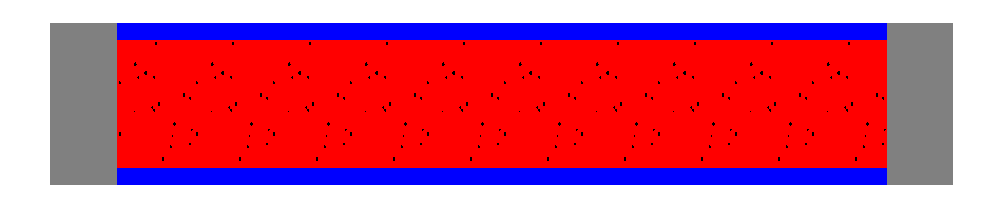
\includegraphics[width=\linewidth]{slab-obj-2-pfppf-min-pf.png}
        \caption{\gls{AHTR} plank model with most-minimized $PF_{total}$
        (corresponds to the orange bolded distribution in Figure 
        \ref{fig:slab-obj-2-pfppf-pareto-distr}).}
        \label{fig:slab-obj-2-pfppf-min-pf} 
    \end{subfigure}
    \begin{subfigure}{\textwidth}
        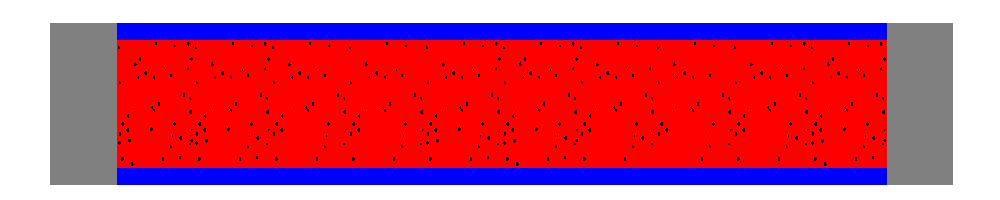
\includegraphics[width=\linewidth]{slab-obj-2-pfppf-min-ppf.png}
        \caption{\gls{AHTR} plank model with most-minimized $PPF_{fuel}$
        (corresponds to the blue bolded distribution in Figure 
        \ref{fig:slab-obj-2-pfppf-pareto-distr}).}
        \label{fig:slab-obj-2-pfppf-min-ppf} 
    \end{subfigure}
    \caption{(contd.) Simulation p-2b -- ROLLO two-objective optimization to minimize 
    total packing fraction ($PF_{total}$) and fuel-normalized power peaking factor 
    ($PPF_{fuel}$) in the plank. 
    Input parameters varied: TRISO packing fraction distribution ($\rho_{TRISO}(\vec{r})$).}
\end{figure}

All reactor models on Figure \ref{fig:slab-obj-2-pfppf}'s Pareto front have a relatively 
flat TRISO packing fraction distribution, varying between 0.02 and 0.04. 
In Figure \ref{fig:slab-obj-2-pfppf-pareto-distr}, the TRISO distribution with the 
most-minimized $PF_{total}$ and highest $PPF_{fuel}$
(the orange distribution) has a constant packing fraction of 0.02 across the plank
(also illustrated in Figure \ref{fig:slab-obj-2-pfppf-min-pf}). 
In Figure \ref{fig:slab-obj-2-pfppf-pareto-distr}, the TRISO distribution with the 
most-minimized $PPF_{fuel}$ and highest $PF_{total}$
(the blue distribution), has a packing fraction that peaks in the center of the plank
and both sides (also illustrated in Figure \ref{fig:slab-obj-2-pfppf-min-ppf}). 
This distribution differs from simulation p-1c's most-minimized $PPF_{fuel}$ TRISO 
distribution (Figure \ref{fig:slab-obj-1-ppf-final}) which has a large $\sim 0.06$ 
variation in TRISO distribution with a minimum point in the center of the plank. 
This difference is due to the different $PF_{total}$ values: simulation p-1c's total PF 
is 0.0979, while the total PF in the most-minimized $PPF_{fuel}$ model 
(blue distribution) is 0.029. 

Figure \ref{fig:flux-comparison-0.0292-plank} compares the flux distributions from the 
Figure \ref{fig:slab-obj-2-pfppf}'s most-minimized $PPF_{fuel}$ TRISO distribution and a 
constant $PF_{total}$ = 0.0292 TRISO distribution. 
The $PPF_{fuel}$ value for constant $PF_{total}$ = 0.292 TRISO distribution is 1.056. 
\begin{figure}[H]
    \centering
    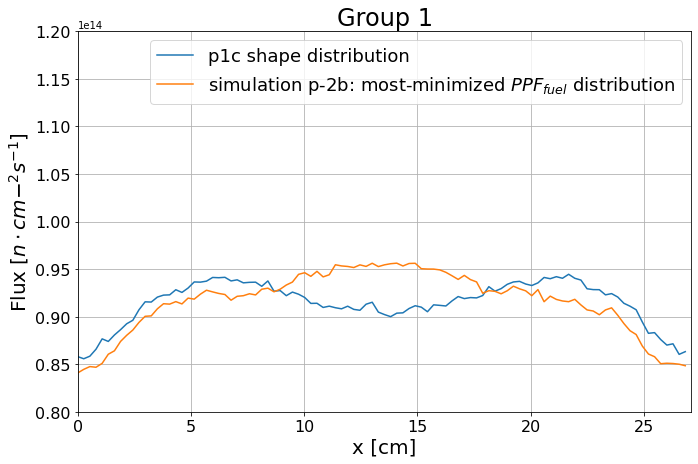
\includegraphics[width=0.48\linewidth]{flux-comparison-0.0292-plank_grp1.png} 
    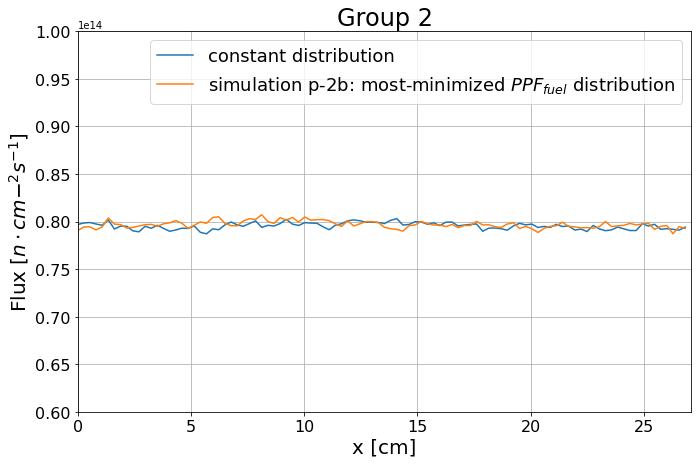
\includegraphics[width=0.48\linewidth]{flux-comparison-0.0292-plank_grp2.png} 
    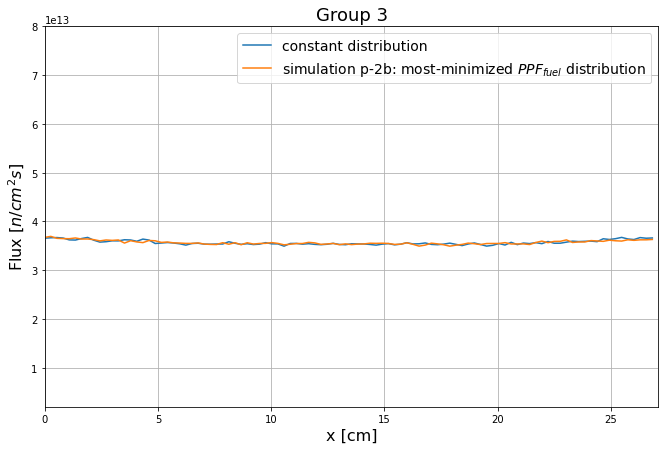
\includegraphics[width=0.48\linewidth]{flux-comparison-0.0292-plank_grp3.png} 
    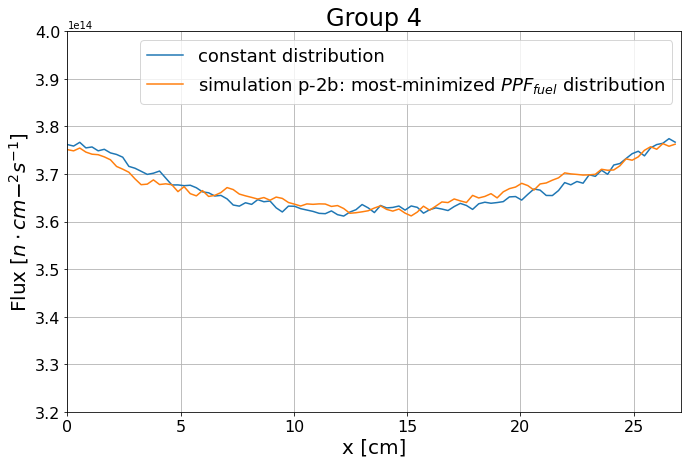
\includegraphics[width=0.48\linewidth]{flux-comparison-0.0292-plank_grp4.png} 
    \caption{Flux comparison between Figure \ref{fig:slab-obj-2-pfppf}'s TRISO 
    distribution that most-minimized $PPF_{fuel}$ and a constant $PF_{total}$ = 0.0292
    TRISO distribution. 
    \acrfull{AHTR} plank's centerline neutron flux distribution in 4 groups at 948K. 
    Centerline is the white line in Figure \ref{fig:ahtr-plank-verification}.
    Energy Group 1: E $> 9.1188 \times 10^{-3}$ MeV, 
    Energy Group 2: $2.9023 \times 10^{-5} < E < 9.1188 \times 10^{-3}$ MeV,
    Energy Group 3:  $1.8556 \times 10^{-5} < E < 2.9023 \times 10^{-5}$ MeV,
    Energy Group 4:  $1.0 \times 10^{-12} < E < 1.8554 \times 10^{-6}$ MeV.}
    \label{fig:flux-comparison-0.0292-plank}
\end{figure}
In Energy group 4, the most-minimized $PPF_{fuel}$ flux distribution is 0.997x flatter 
than the constant $PF_{total}$ = 0.0292 flux distribution, resulting in a lower 
$PPF_{fuel}$. 

Theory: The $PF_{total}$ = 0.0979 TRISO distribution has more self-shielding, therefore, 
a larger variation in TRISO distribution flattens thermal flux more than the 
$PF_{total}$ = 0.0292. 
$PF_{total}$ = 0.0292 does not require such a large TRISO variation. 
In Group 4, $PF_{total}$ = 0.0979 TRISO distribution has 
$\frac{Max(Flat Flux)}{Min(Flat Flux)} = 1.115$ while $PF_{total}$ = 0.0292 TRISO 
distribution has $\frac{Max(Flat Flux)}{Min(Flat Flux)} = 1.045$, proving that the 
former has more thermal flux self-shielding. 

Minimize $PPF_{fuel}$ objective is driven by flattening thermal (Group 4) flux.

\pagebreak
\section{Understanding Minimize $PF_{total}$}

\subsubsection{Simulation p-1a: Variation of $\rho_{TRISO}(\vec{r})$ and $PF_{total}$ 
to minimize $PF_{total}$}
Table \ref{tab:simulationp1a} shows simulation p-1a's optimization problem parameters. 
\begin{table}[htbp!]
    \centering
    \onehalfspacing
    \caption{Simulation p-1a optimization problem parameters.}
	\label{tab:simulationp1a}
    \footnotesize
    \begin{tabular}{l|p{5cm}}
    \hline 
    \multicolumn{2}{c}{\textbf{Single Objective: Simulation p-1a}} \\
    \hline 
    \textbf{Objectives} & Minimize $PF_{total}$ \\
    \hline 
    \textbf{Input parameter variations} & $0.02<PF_{total}<0.04$ \\
    & $0<a<2$ \\
    & $0<b<\frac{\pi}{2}$ \\
    & $0<c<2\pi$ \\
    \hline
    \textbf{Constraints} & $k_{eff} \geq 1.35$\\ 
    \hline 
    \textbf{Genetic algorithm parameters} & Population size: 60 \\
    & Generations: 10 \\
    \hline
    \end{tabular}
\end{table}

Figure \ref{fig:slab-obj-1-pf-evol} shows the $PF_{total}$ evolution,  
Figure \ref{fig:slab-obj-1-pf-final} shows the five TRISO packing fraction 
distributions ($\rho_{TRISO}(\vec{r})$) in the final generation with the 
most-minimized $PF_{total}$, and Figure \ref{fig:slab-obj-1-pf-most-minimized} 
illustrates the \gls{AHTR} plank model with most-minimized $PF_{total}$.
\begin{figure}[htbp!]
    \centering
    \begin{subfigure}{0.95\textwidth}
        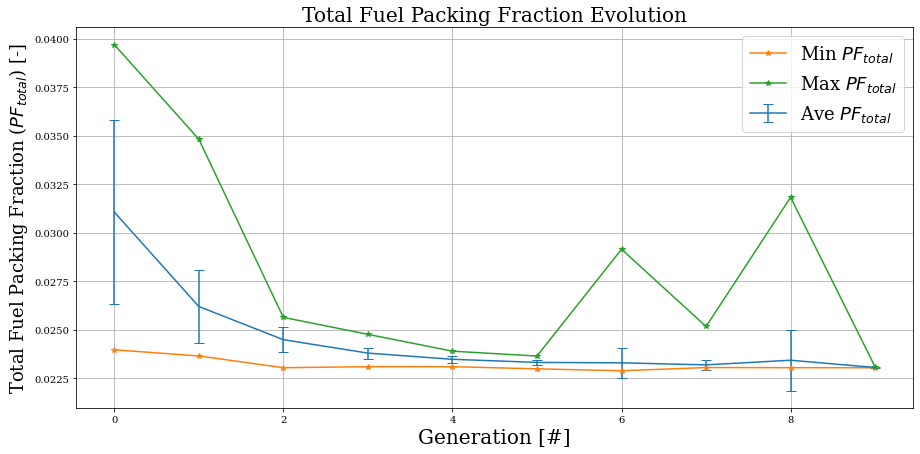
\includegraphics[width=\linewidth]{slab-obj-1-pf-evol.png}
        \caption{Minimum, average, and maximum $PF_{total}$ evolution.}
        \label{fig:slab-obj-1-pf-evol} 
    \end{subfigure}
    \begin{subfigure}{0.95\textwidth}
        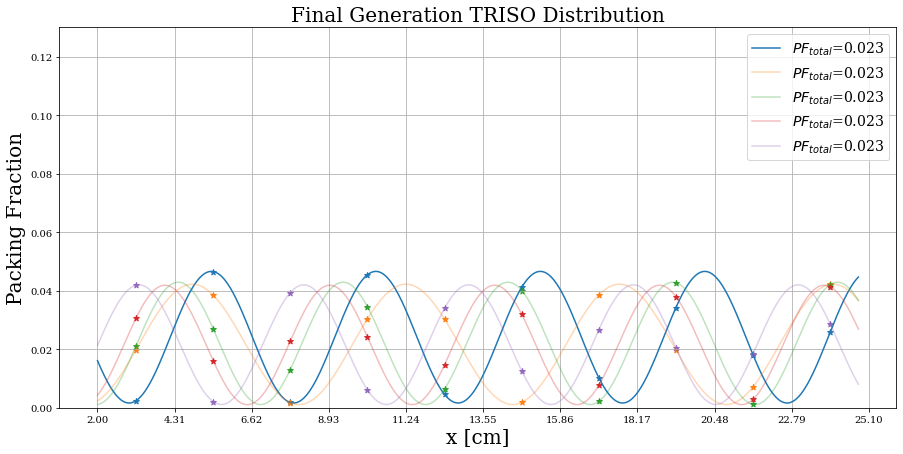
\includegraphics[width=\linewidth]{slab-obj-1-pf-final.png}
        \caption{TRISO packing fraction distribution for the 5 reactor models with the 
        smallest $PF_{total}$ in the final generation.}
        \label{fig:slab-obj-1-pf-final} 
    \end{subfigure}
    \begin{subfigure}{0.95\textwidth}
        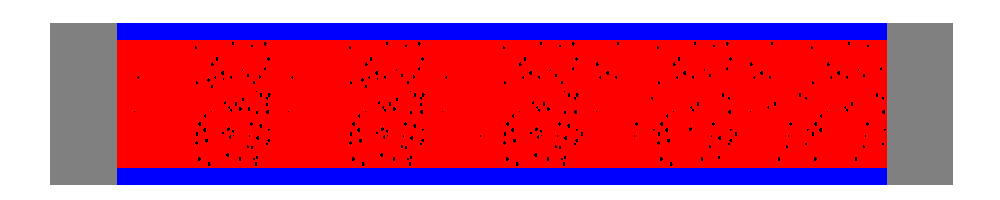
\includegraphics[width=\linewidth]{slab-obj-1-pf-most-minimized.png}
        \caption{\gls{AHTR} plank model with most-minimized $PF_{total}$ 
        (corresponds to the blue bolded distribution in the above plot).}
        \label{fig:slab-obj-1-pf-most-minimized} 
    \end{subfigure}
    \caption{Simulation p-1a -- ROLLO single-objective optimization to minimize total 
    fuel packing fraction. Input parameters varied: total fuel packing fraction 
    ($PF_{total}$), \gls{TRISO} packing fraction distribution ($\rho_{TRISO}(\vec{r})$).}
    \label{fig:slab-obj-1-pf}
\end{figure}

I ran a simulation for constant $PF_{total}$ = 0.023. 
Figure \ref{fig:flux-comparison-0.023-plank} compares the flux distributions from the 
Figure \ref{fig:slab-obj-1-pf}'s most-minimized $PF_{total}$ TRISO distribution and a 
constant $PF_{total}$ = 0.023 TRISO distribution. 
\begin{figure}[H]
    \centering
    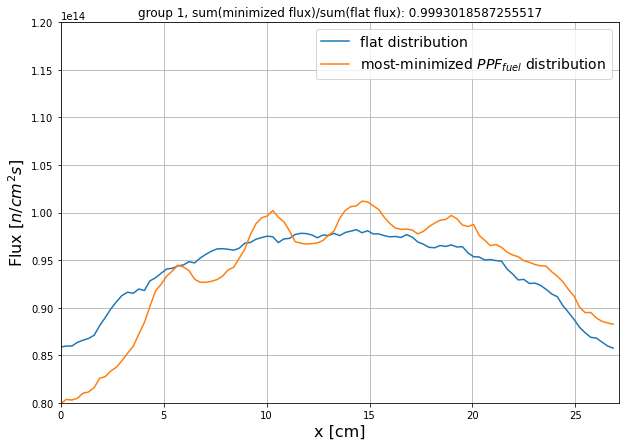
\includegraphics[width=0.48\linewidth]{flux-comparison-0.023-plank_grp1.png} 
    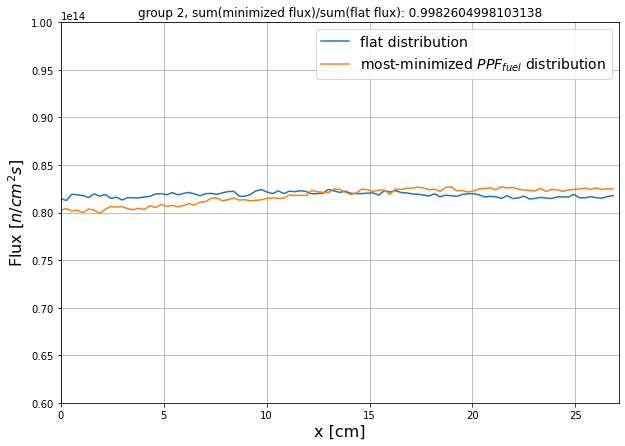
\includegraphics[width=0.48\linewidth]{flux-comparison-0.023-plank_grp2.png} 
    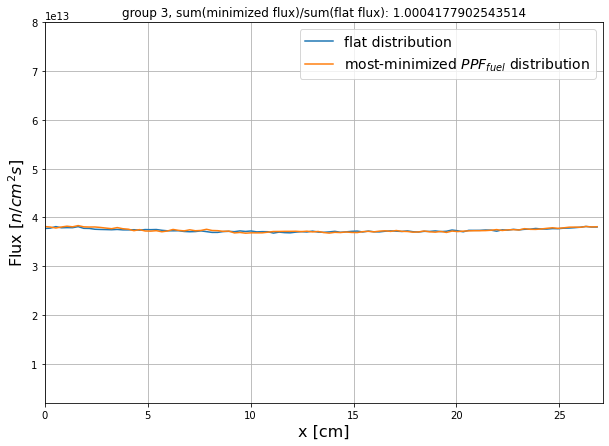
\includegraphics[width=0.48\linewidth]{flux-comparison-0.023-plank_grp3.png} 
    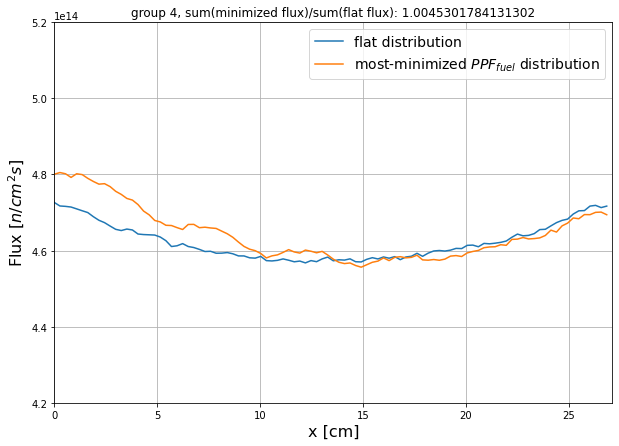
\includegraphics[width=0.48\linewidth]{flux-comparison-0.023-plank_grp4.png} 
    \caption{Flux comparison between Figure \ref{fig:slab-obj-1-pf}'s TRISO 
    distribution that most-minimized $PF_{total}$ and a constant $PF_{total}$ = 0.023
    TRISO distribution. 
    \acrfull{AHTR} plank's centerline neutron flux distribution in 4 groups at 948K. 
    Centerline is the white line in Figure \ref{fig:ahtr-plank-verification}.
    Energy Group 1: E $> 9.1188 \times 10^{-3}$ MeV, 
    Energy Group 2: $2.9023 \times 10^{-5} < E < 9.1188 \times 10^{-3}$ MeV,
    Energy Group 3:  $1.8556 \times 10^{-5} < E < 2.9023 \times 10^{-5}$ MeV,
    Energy Group 4:  $1.0 \times 10^{-12} < E < 1.8554 \times 10^{-6}$ MeV.}
    \label{fig:flux-comparison-0.023-plank}
\end{figure}

Table \ref{tab:0.023-plank-fission-rate} compares the \texttt{fission} 
(total fission reaction rate) between the most-minimized $PF_{total}$ TRISO 
distribution and a constant $PF_{total}$ = 0.023 TRISO distribution.
\begin{table}[H]
    \centering
    \onehalfspacing
    \caption{\texttt{fission} (total fission reaction rate) comparison 
    between the most-minimized $PF_{total}$ TRISO distribution and a constant 
    $PF_{total}$ = 0.023 TRISO distribution.}
	\label{tab:0.023-plank-fission-rate}
    \footnotesize
    \begin{tabular}{llp{4cm}p{4cm}p{5cm}}
    \hline
    \textbf{Group} & 
    \textbf{$\%$ of Total} &
    \textbf{Most-minimized $PF_{total}$ fission} & 
    \textbf{Flat $PF_{total}$ fission} & 
    \textbf{sum(most-minimized $PF_{total}$ fission) / sum(flat $PF_{total}$ fission)}\\
    \hline 
    1 & 0.21 & 0.001260 & 0.001234 & 1.0207 \\
    2 & 1.16 & 0.006653 & 0.006658 & 0.9992 \\
    3 & 1.15 & 0.006566 & 0.006580 & 0.9978 \\
    4 & 97.44 & 0.556897 & 0.555889 & 1.0018 \\
    \hline
    \end{tabular}
\end{table}

Table \ref{tab:0.023-plank-nu-fission-rate} compares \texttt{nu-fission} (total 
production of neutrons due to fission) between the most-minimized $PF_{total}$ TRISO 
distribution and a constant $PF_{total}$ = 0.023 TRISO distribution.
\begin{table}[H]
    \centering
    \onehalfspacing
    \caption{\texttt{nu-fission} (total production of neutrons due to fission) comparison 
    between the most-minimized $PF_{total}$ TRISO distribution and a constant 
    $PF_{total}$ = 0.023 TRISO distribution.}
	\label{tab:0.023-plank-nu-fission-rate}
    \footnotesize
    \begin{tabular}{llp{4cm}p{4cm}p{5cm}}
    \hline
    \textbf{Group} & 
    \textbf{$\%$ of Total} &
    \textbf{Most-minimized $PF_{total}$ nu-fission} & 
    \textbf{Flat $PF_{total}$ nu-fission} & 
    \textbf{sum(most-minimized $PF_{total}$ nu-fission) / sum(flat $PF_{total}$ nu-fission)}\\
    \hline 
    1 & 0.23 & 0.003275 & 0.003206 & 1.0216 \\
    2 & 1.16 & 0.016198 & 0.016210 & 0.9992 \\
    3 & 1.15 & 0.016000 & 0.016034 & 0.9978 \\
    4 & 97.44& 1.356992 & 1.354534 & 1.001 \\
    \hline
    \end{tabular}
\end{table}

Minimize $PF_{total}$ objective is driven by maximizing total fission reaction rate in 
thermal energy group (Group 4). 